\chapter{Test Bed}
\label{chp:testbed}
We setup our testbed in an $8m\times6m$ office space. Sensors are mounted on the ceiling which is at a height of 3m. The sensors are  placed 2.5m apart in the horizontal direction and 2.2m apart in the vertical direction. A schematic representation of the lab is as shown in the Figure \ref{fig:roomLayout} with the positions of the sensors marked. We use  PIR sensor, EKMB1101112 from Panasonic. 
The output of the sensor is binary, with 1 indicating occupancy and 0 if the region is unoccupied.  We use the sensors with eZ430-RF2500 toolkit which consists of MSP430 micro-controller  and CC2500 multi-channel
RF transceiver for wireless communication. The testbed uses simpliciTI a TI proprietary  low-power RF network protocol.  We mount all the 8 sensors on the ceiling of the room as shown in the Figure \ref{fig:photo}. 
All the 8 nodes communicate directly to a centrally located access point which is connected to a laptop, which stores the data.

\begin{figure}[!ht]
\centering
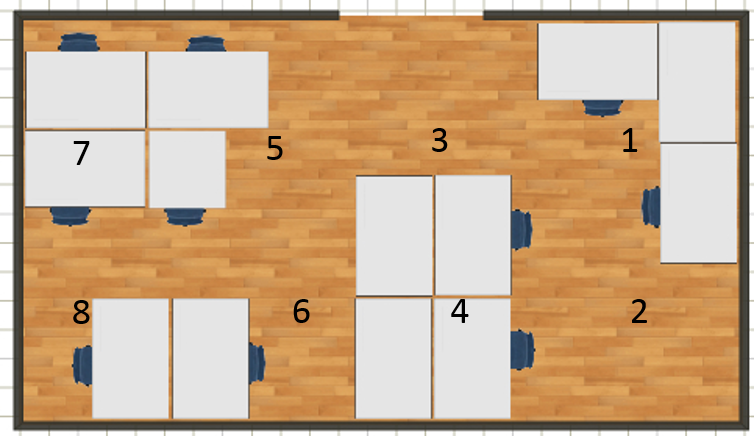
\includegraphics[scale=0.5]{./pics/roomLayout.png}
\caption{Room layout of the testbed.}
\label{fig:roomLayout}
\end{figure}


\begin{figure}[!ht]
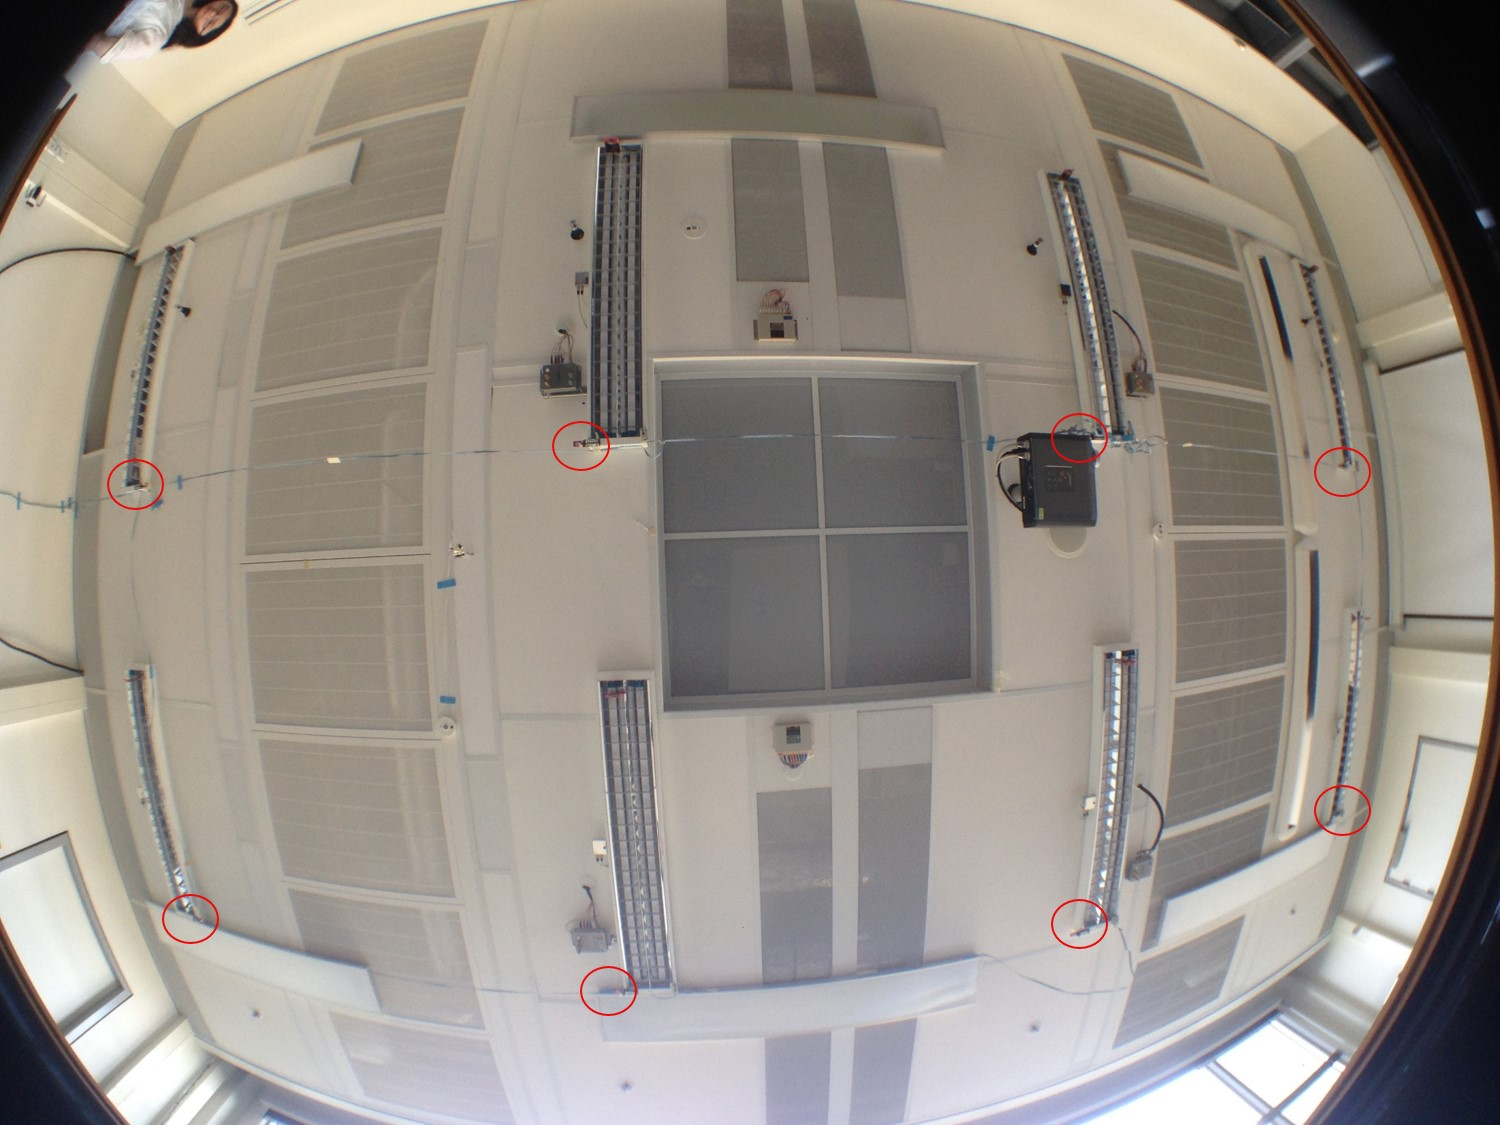
\includegraphics[scale=0.5]{./pics/lab_photo.jpg}
\caption{Photo of the lab setup with the sensors highlighted in red}
\label{fig:photo}
\end{figure}

\section{Packet Loss}
To avoid collision between the transmitted packets CSMA/CA is employed in our testbed. Even though CSMA/CA is employed, during our initial tests we observed packet loss as high as 23\% for few nodes as shown in the Figure \ref{fig:ackDis} and Table \ref{tab:packetLoss}. To decrease the packet loss we enable acknowledgment. An acknowledgment (ack) is sent from the AP if the packets are received. If no ack is received by a node, the node retransmits its data a maximum of 5 times until an ack is  received from the AP. If no ack is received even after 5 retransmission the packet is dropped and the next packet is prepared for transmission. From the Figure \ref{fig:ackEnb} and Table \ref{tab:packetLoss} we can see that the there was a decrease in the packet loss per node after ack was enabled. 

\begin{figure}[!ht]
    \centering
    \begin{subfigure}[b]{1\textwidth}
        \centering
        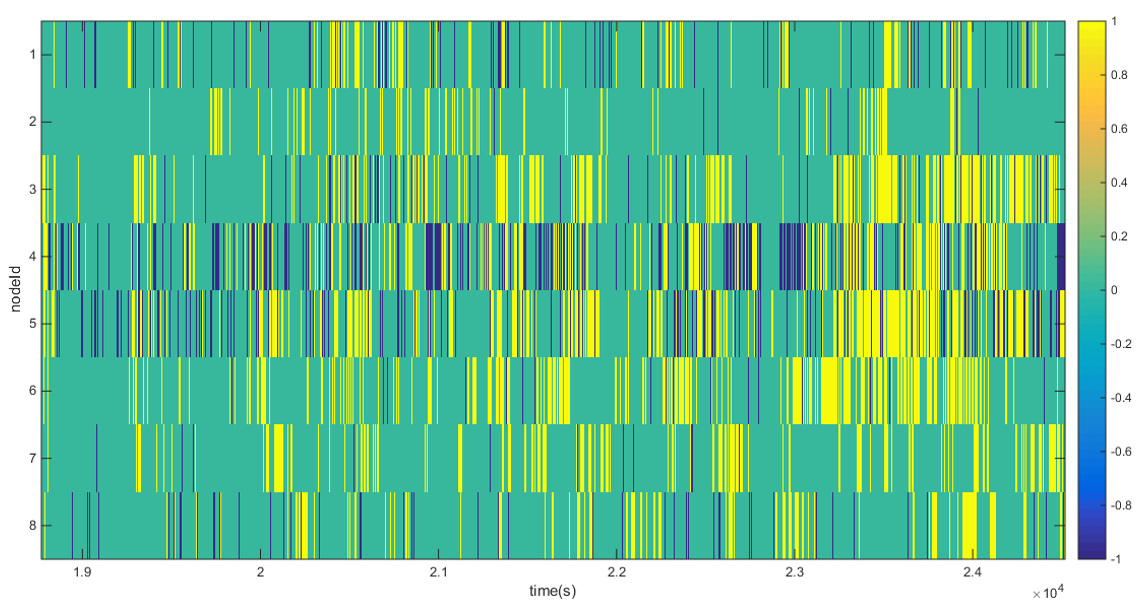
\includegraphics[width=8cm,height=4cm]{./pics/packetLoss.png}
      \caption{Data before ack was enabled}
       \label{fig:ackDis}
    \end{subfigure}
    \hfill
    \begin{subfigure}[b]{1\textwidth}
        \centering
        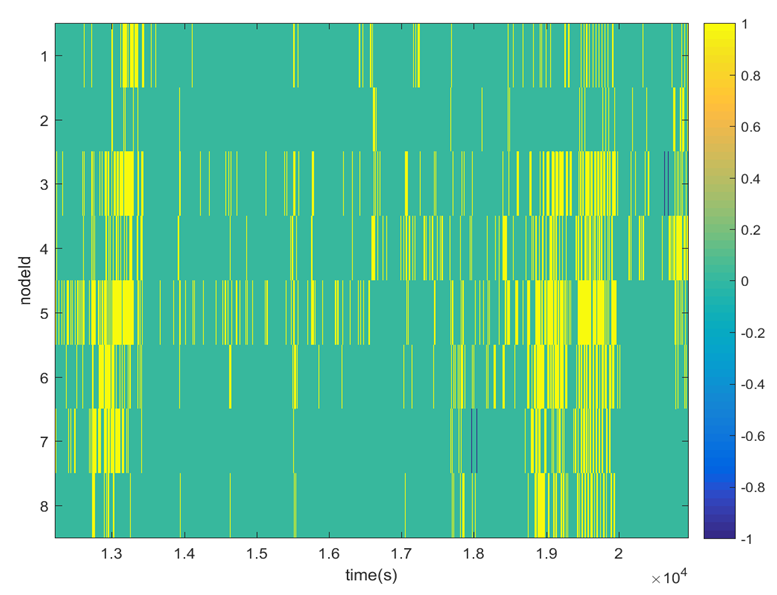
\includegraphics[width=8.5cm,height=4cm]{./pics/dataAfterAck.png}
        \caption{Data after ack was enabled}
        \label{fig:ackEnb}
    \end{subfigure}
\caption{Data from the test bed. - 1 indicates the lost data , 1 indicates occupancy, 0 indicates unoccupied space}
\label{fig:packetLoss}
\end{figure}

\begin{table}[!ht]
\centering
\caption{Packet loss without and with ack for all the sensor nodes}
\label{tab:packetLoss}
\begin{tabular}{|c|c|c|}
\hline
Node & \begin{tabular}[c]{@{}c@{}}Packet loss Without \\ ack(\%)\end{tabular} & Packet loss With ack(\%) \\ \hline
1    & 7.66                                                               & 0                    \\ \hline
2    & 1.01                                                             & 0                    \\ \hline
3    & 5.65                                                             & 0.32                 \\ \hline
4    & 23.67                                                            & 0                    \\ \hline
5    & 14.05                                                            & 0                    \\ \hline
6    & 1.48                                                             & 0                    \\ \hline
7    & 0.96                                                              & 2.20                    \\ \hline
8    & 4.54                                                             & 0                    \\ \hline
\end{tabular}
\end{table}


\section{Time synchronization}
In our testbed, each sensor node has a local clock running on it, with each clock tick corresponding to 1ms. Environment fluctuations, difference in battery levels or imperfection in clock construction can result in one of the clocks ticking faster than the other. To overcome this drift between the clocks we implement one-way synchronization as explained in \cite{kerkez2012adaptive}. In this method, all the local clocks are synchronized to a centrally located node which has a clock running on it. This node transmits the packets periodically after every minute, containing the timestamp corresponding to the local time on the node. The sensor node upon receiving the packets set their local clock to the time specified in the received packet. 
\begin{figure}[!ht]
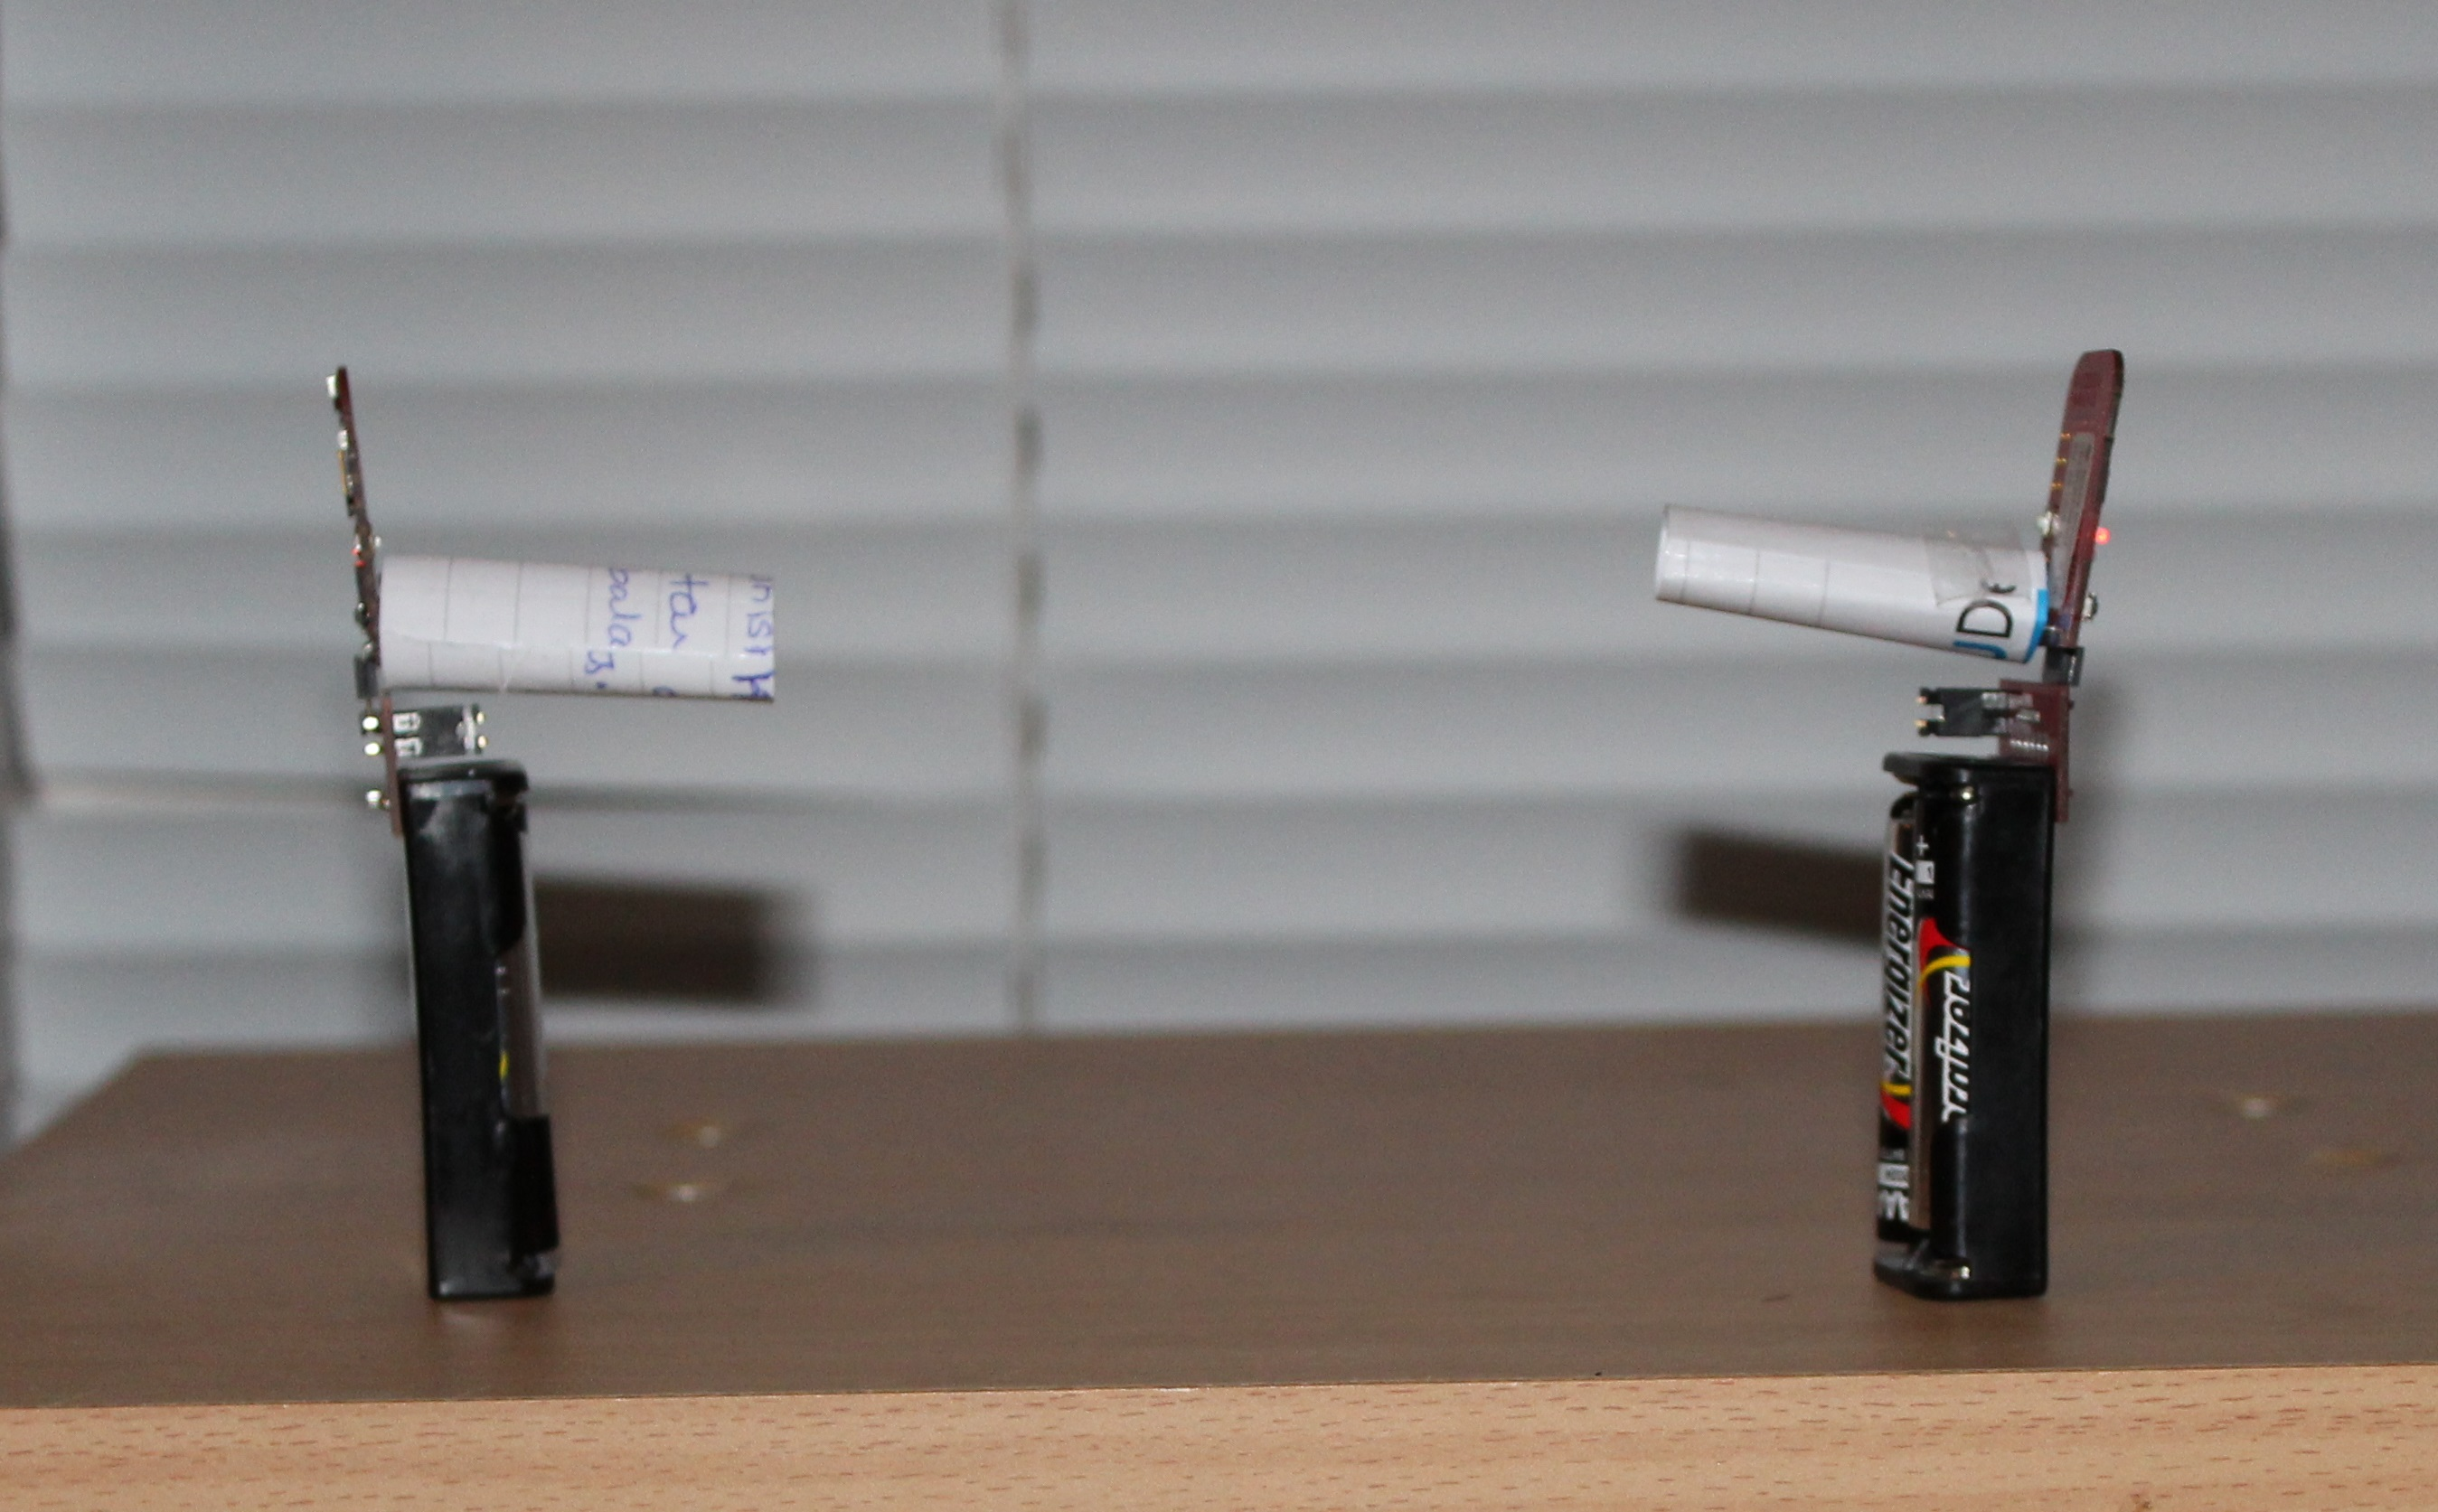
\includegraphics[scale=0.1]{./pics/timesync.jpg}
\caption{Setup to test time synchronization}
\label{fig:timeSync}
\end{figure}

\begin{figure}
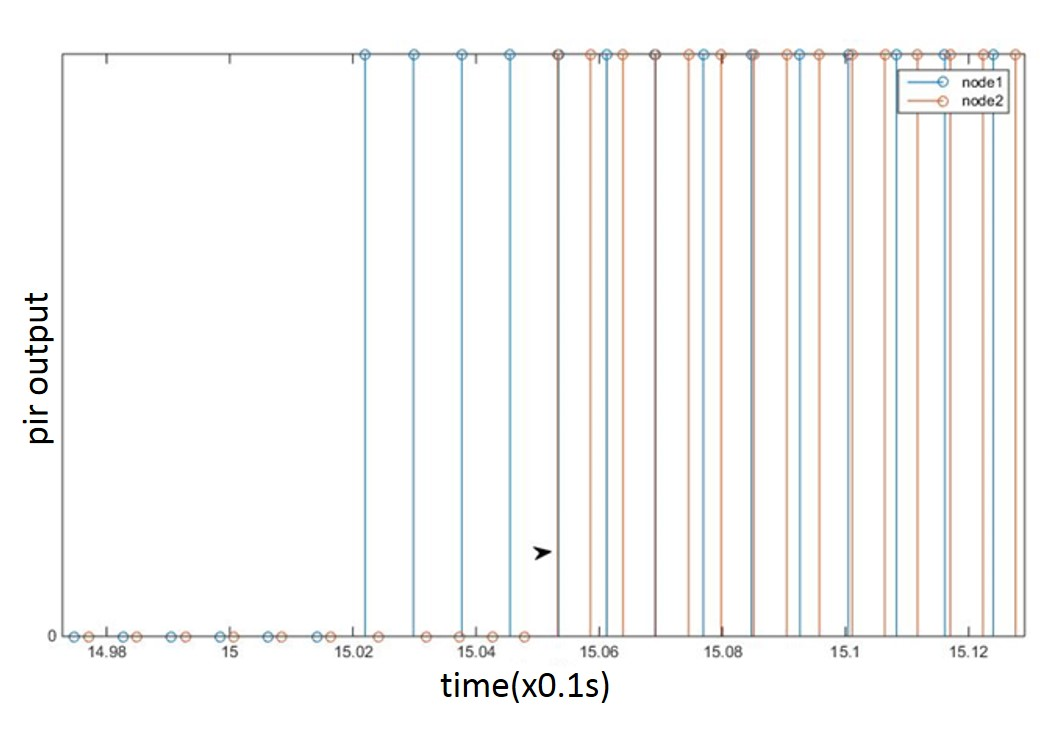
\includegraphics[scale=0.5]{./pics/timeSyncErr}
\caption{Worst case time synchronization error between two nodes}
\label{fig:timeSyncErr}
\end{figure}

To test the time synchronization we place two sensor nodes opposite to each other as shown in the Figure \ref{fig:timeSync}. We sample the sensors at 10ms. To limit the field of view of the sensors we cover the sensor with paper roll. We introduce an obstacle swiftly between the sensor for a short period. This process is repeated 10 times and the worst case time synchronization error is as shown in the Figure \ref{fig:timeSyncErr}. As can be seen in the figure the worst case time synchronization error is approximately equal to 40ms, which is acceptable for our application.

\section{Packet Structure}
In our testbed, we sample our occupancy sensors once every 100ms. Since the data is binary we combine 32 samples and transmit the packet every 3.2s. This decreases the traffic in the sensor network.
The transmitted packet is an array of unsigned integer of size one byte. Consisting of 14 bytes of payload. The payload structure is as shown in the Figure \ref{fig:packetStructure}
\begin{figure}[!ht]
 \bytefieldsetup{bitheight=3em}
\begin{bytefield}[bitwidth=2.5em]{14}
\bitheader{0-13} \\
\bitbox{1}{\tiny Mac id} & \bitbox{1}{\tiny packet number} &
\bitbox{4}{start time}
& \bitbox{4}{end time} & \bitbox{4}{data}
\end{bytefield}.
\caption{Packet Structure}
\label{fig:packetStructure}
\end{figure}

\begin{itemize}
\item Mac Id - unique identifier for each node. Mac Id is used to assign the packets received to the particular node. 
\item Packet number- Keeps track of the packets that are being transmitted from a  node. It helps to identify the lost packets as well as repeated packets. If two packets from the same node have the same packet number then they are treated as duplicate packets. If there is a packet number missing then we treat that as a lost packet.
\item Start time - 4 byte array corresponding to the time of first occupancy sensor sample in the packet.  
\item End time - 4 byte array corresponding to the time of the last occupancy sensor sample in the packet.
\item Data - 4 byte array which is combined and converted to binary form. This represents 32 samples of the occupancy sensor output. Each sample separated by an interval of 100ms. 
\end{itemize}
\section{Data Collection}
Data was collected for a span of 2 months. During the course of the evaluation, the occupants were notified of data gathering, but were never instructed to behave in any particular way or was there any constrained applied on the activity or the number of people in the room. All nodes directly communicated to a centrally located AP, which was connected to a laptop which was used to store the data. We collected a total of approximately 120hrs of data. Figure \ref{fig:dataFig} shows a part of the binary data obtained from the testbed.
\begin{figure}[!ht]
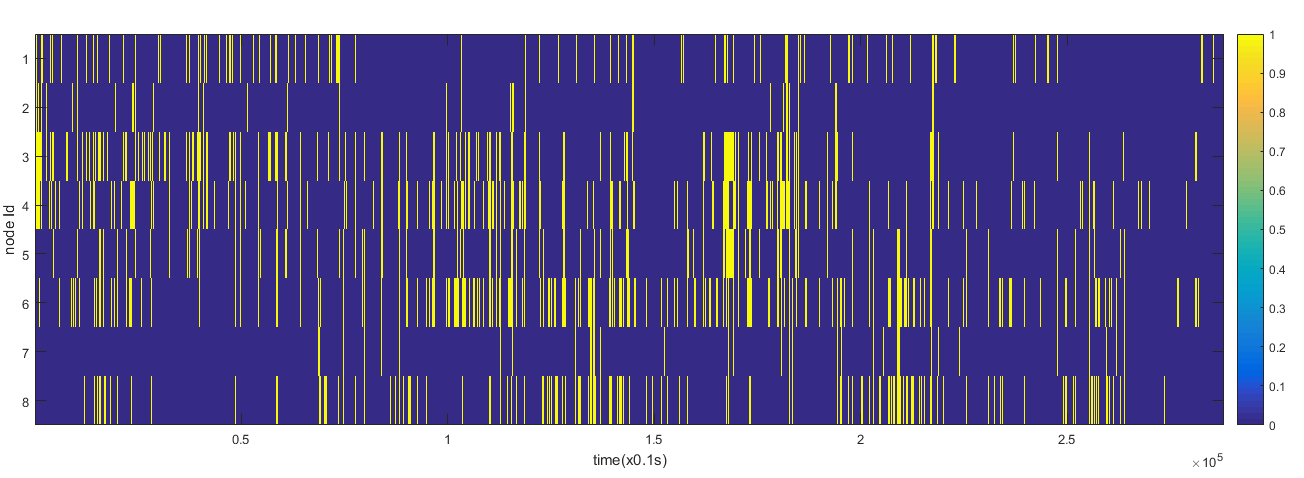
\includegraphics[width=\textwidth]{./pics/data.png}
\caption{Binary data obtained from the testbed spanning for 8hrs}
\centering
\label{fig:dataFig}
\end{figure}



